\documentclass[a4paper,11pt]{article}

\usepackage{a4wide}
\usepackage{graphicx}
\usepackage{moreverb}
\usepackage{hyperref}

\title{PeerSim HOWTO:\\ Build a new protocol for the PeerSim 1.0 simulator}
\author{Gian Paolo Jesi (jesi@cs.unibo.it)}

\begin{document}

\maketitle


\noindent\emph{This tutorial is for PeerSim 1.0, in particular, its so called
cycle based engine.
If the reader is not a PeerSim newbie, she may be
interested in what major changes have been introduced since the last version.
The changes are summarized in Appendix~\ref{sec:Appendix-C-changes}.
For all the details, check the PeerSim CHANGELOG file, included in the
distribution.}

\section{Introduction}


This tutorial is a step by step guide to build from
scratch a new PeerSim application.
In this tutorial it is supposed that you have access to: 

\begin{itemize}
\item knowledge of the Java language
\item a Java compiler for Java version 1.5; we propose $\geq$ JDK 1.5.x
\item the PeerSim 1.0 package (\url{http://sourceforge.net/projects/PeerSim}), 
or the PeerSim source tree (you can download it from the sourceforg CVS server)
\item the Java Expression Parser version $\geq$ 2.3.0
(included in the release, but you can download it from
\url{http://www.singularsys.com/jep/})
\item the gnuplot plotting tool is highly recommened 
\end{itemize}

The aim of this tutorial is inteded to be
as practical and lightweight as possible.
The goal is to give the reader the basics
of PeerSim usage and the basics about how to write a simple protocol,
through a step-by-step example.
This tutorial IS NOT exhaustive at all, it is not meant to be a comprehensive
guide, but it is enough to get you started.


\section{Introduction to Peersim}


\subsection{Why PeerSim}

Peer-to-peer (P2P) systems can be extremely large
scale (millions of nodes).
Nodes in the network join and leave continuously.
Experimenting with a protocol in such an environment it no easy task at all.

Peersim has been developed to cope with these properties and thus
to reach extreme scalability and to support dynamism. In addition,
the simulator structure is based on components and makes it easy to quickly
prototype a protocol, combining different pluggable building
blocks, that are in fact Java objects.

PeerSim 1.0 supports two simulation models: the so called cycle-based model
and the traditional event based model.
This document is about the cycle based model.
This model is a simplifed model, which makes it possible to achieve extreme
scalability and impressive performance, at the cost of some loss of realism.
Many protocols can tolerate this loss of realism very well, according to
our onw research; however,
care should be taken when this model is selected to experiment with a protocol.

The simplifying assumptions of the cycle based model are the lack of
transport layer simulation and the lack of concurrency.
In other words, nodes communicate with each other directly, and the nodes
are given the control periodically, in some sequential order, when they can
perform arbitrary actions, such as call methods of other objects and perform
some computations.

We note here that it is realtively easy to migrate any cycle-based simulations
to the event driven engine. However, we don't discuss how to do it in this
document.

\subsection{Peersim simulation life-cycle}

PeerSim was designed to encourage modular programming based on objects
(building blocks). Every such block is easily replaceable by another component
that has a similar function, that is, that  has the same interface.
The general idea of the simulation model is:

\begin{enumerate}
\item choose a network size (number of nodes) 
\item choose one or more protocols to experiment with and initialize
them
\item choose one or more \emph{Control} objects
  to monitor the properties
  you are interested in and to modify some parameters during
  the simulation (e.g., the size of the
 network, the internal state of the protocols, etc) 
\item run your simulation invoking the \emph{Simulator} class with a
configuration file, that contains the above information
\end{enumerate}

All the object created during the simulation are instances of classes
that implement one or more interfaces. The
main interfaces to become familiar with are listed in
Table~\ref{t:psim_classes}.


\label{table1}
\begin{table}
\begin{center}\begin{tabular}{|l|p{11cm}|}
\hline 
\emph{Node}&
The P2P network is composed of nodes. A node is a container of
protocols. The node interface provides access to the protocols
it holds, and to a fixed ID of the node.\\
\hline 
\emph{CDProtocol}&
It is a specific protocol, that is designed to run in the cycle-driven
model. Such a protocol simply defines an operation to be performed at
each cycle.\\
\hline 
\emph{Linkable}&
Typically implemented by protocols, this interface provides a service
to other protocols to access a set of neighbor nodes.
The instances of the same linkable protocol class over the nodes define
an overlay network.\\
\hline 
\emph{Control}&
Classes implementing this interface can be scheduled for execution at
certain points during the simulation.
These classes typically observe or
modify the simulation.\\
\hline
\end{tabular}\end{center}

\caption{\label{t:psim_classes}Suggested PeerSim subset of classes or
  interfaces to know about.} 
\end{table}


The life-cycle of a cycle-based simulation is as follows.
First the configuration file is read, that is given as a command line
parameter (see section 
\ref{configfile}).
The configuration contains all the simulation parameters 
concerning all the
objects involved in the experiment.

Then the simulator sets up the network initializing the nodes in the
network, and the protocols in them.
Each node has the same kinds of protocols; that is, instances of
a protocols form an array in the network, with one instance in each
node.
The instances of the nodes and the protocols are created by cloning.
That is, only one instance is constructed using the constructor of the
object, which serve as prototypes, and all the nodes in the network are
cloned from this prototype.
For this reason, it is very important to play attention to the implementation
of the cloning method of the protocols.

At this point, initialization needs to be performed, that sets up the
initial states of each protocol.
The initialization phase is carried out by \emph{Control}
objects that are scheduled to run only at the beginning of each experiment.
In the configuration file,
the initialization components are easily recognizable by the
\texttt{init} prefix. Please note that in the following pages we will
talk about \emph{Initializer} objects just to remark their function and
to distinguish them from ordinary \emph{Control} objects, but the initializer
objects are simply controls, configured to run in the initialization phase.

After initialization, the cycle driven engine calls all components (protocols
and controls) once in each cycle, until a given number of cycles, or until
a component decides to end the simulation.
Each object in PeerSim (controls and protocols) is assigned a
\emph{Scheduler} object which defines when they are executed exactly.
By default, all objects are executed in each cycle.
However, it is possible to configure a protocol or control to run only in
certain cycles, and it is also possible to control the order of the running
of the components within each cycle.
The latter scenario is illustrated in Figure~\ref{obsfigure}. 


\begin{figure}
\begin{center}
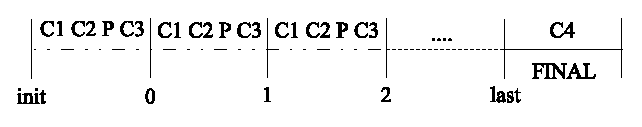
\includegraphics[scale=1.1]{controls-protocols}
\end{center}
\caption{Scheduling controls and protocols. The ``C'' letters indicate a
  control component, while letter ``P'' indicates a protocol.
  The numbers in lower part of the picture indicate the
  PeerSim cycles. After the last cycle, it is possible to run a final
  control to retrieve a final snapshot.\label{obsfigure}}
\end{figure}


When a \emph{Control} has to collect data, they are formatted and sent to
standard output and can be easily redirected to a file to be collected
for further work. 
%When developing such a \emph{Control} class, a good
%rule is to print out data using the \emph{PeerSim.core.Log} static class.


\subsection{The config file}
\label{configfile}

The config file is a plain ASCII text file, basically composed of
key-value pairs; the lines starting with \char`\"{}\#\char`\"{} character
are ignored (comments). The pairs are collected by a standard Java
\emph{java.util.Properties} object when the simulator starts using
for example the following command:

\begin{verbatim}
java -cp <class-path> PeerSim.Simulator config-file.txt \end{verbatim}


Clearly the classpath is mandatory only if you have not set it yet
in a global shell variable.

\subsection{Configuration example 1}

We are going to create a fixed P2P random topology composed of 50000
nodes.
The chosen protocol is \emph{Aggregation} (what is
aggregation? see appendix \ref{sec:Appendix-A-aggregation}) using
the average function. The values to be aggregated (averaged) at each
node are initialized using a linear distribution on the interval (0,
100). Finally a \emph{Control} monitors the averaging values.
Looks easy!

\footnotesize
\begin{listing}{1}
# PEERSIM EXAMPLE 1

random.seed 1234567890
simulation.cycles 30

control.shf Shuffle

network.size 50000
 
protocol.lnk IdleProtocol

protocol.avg example.aggregation.AverageFunction
protocol.avg.linkable lnk
 
init.rnd WireKOut
init.rnd.protocol lnk
init.rnd.k 20

init.peak example.aggregation.PeakDistributionInitializer
init.peak.value 10000
init.peak.protocol avg

init.lin LinearDistribution
init.lin.protocol avg
init.lin.max 100
init.lin.min 1

# you can change this to select the peak initializer instead
include.init rnd lin

control.avgo example.aggregation.AverageObserver
control.avgo.protocol avg
\end{listing}

\normalsize


The first things to note are the
key names: some of them refer to global properties, while some
others refer to single component instancies. For example,
\texttt{simulation.cycles} is global, but \texttt{protocol.lnk.xxx}
defines parameter \textbf{xxx} of protocol \textbf{lnk}.

Observe that each component has a name,
such as \texttt{lnk}. In the case of protocols, this
name is mapped to a numeric index called protocol ID, by the PeerSim
engine.
This index does not appear in the configuration file, but it is necessary
to access protocls during a simulation.
We give more details later.

A component such as a protocol or a control is declared by  the
following syntax:

\begin{verbatim} <protocol|init|control>.string_id [full_path_]classname
\end{verbatim}

Note that the full class path is optional, in fact PeerSim can search
in its classpath in order to find a class. If multiple classes share
the same name (in distinct packages), the full path is needed.
The prefix {\tt init} defines an initializer object, that has to implement
the Control interface.
  
The component parameters (if any) follows this scheme:

\begin{verbatim} <protocol|init|control>.string_id.parameter_name
\end{verbatim}

For example, at \textbf{line 10}, the first protocol chosen comes to life;
the \textbf{key part} contains its type, in this case {\tt protocol}
followed by the name, in this case {\tt lnk}, and \textbf{the
value} part contains the classname for the component, in this case
{\tt IdleProtocol}.
This class is in the peersim package, and you don't have to know what is
its fully specified name.

Parameters can be declared for each component.
For example, see \textbf{line 13}, where the \textbf{key part} contains the
parameter name and the \textbf{value part} is simply the value desired.

From \textbf{line 3 to line 8}
some global simulation properties are imposed; these are the total
number of simulation cycles and the overlay network size. The
\emph{Shuffle} control (\textbf{line 6}) shuffles the order in which the nodes
are visited in each cycle. 

From \textbf{line 10 to line 13}, two protocols are put in the arena.
The first one, \emph{IdleProtocol} does nothing.
It simply serves as a static container of links to neighboring nodes.
The class \emph{IdleProtocol} does not implement \emph{CDProtocol}, but it
does implement the \emph{Linkable} interface, through which it provides
the links to neighbors.

The second protocol (\texttt{protocol.avg aggregation.AverageFunction})
is the averaging version of aggregation. Its parameter (\texttt{linkable})
is important: the aggregation protocol needs to talk to neighbors
but doesn't have its own list of neighbors.
In a modular fashion, it can be put over any overlay network.
The protocol (array) that defines the overlay network has to be specified
here.
The value of parameter linkable is the name
of a protocol implementing  the \emph{Linkable} interface
(\emph{IdleProtocol}
in the example).

From \textbf{line 15 to line 26}, it is time to initialize all the
components previously declared. We declare three initialization components,
but only two of them are actually used (see \textbf{line 29}).
The first initializer, \texttt{PeerSim.init.WireKOut},
performs the wiring of the static overlay network. 
In particular, the nodes are linked
randomly to each-other to form a random graph having the specified
degree (\texttt{k}) parameter. 

The second and third initializers are alternatives to initialize the aggregation
protocol, in particular, the initial values to be averaged.
The initializaters set the initial values to follow a peak or linear
distribution, respectively.
Peak means that only one node will have a value different from zero.
Linear means that the nodes will have linearly increasing values.
Both initializers need a protocol name that identifies the
protocol to initialize (\texttt{protocol} parameter).
Additional parameters are the range (\texttt{max}, \texttt{min}
parameters)
for the \emph{PeakDistributionInitializer} and \texttt{value}
parameter for \emph{LinearDistribution}. 

The choice to use the peak or linear distribution is given by the
\texttt{include.init} property (\textbf{line 29}) that selects which
initializers are 
allowed to run.
This property also defines the order in which the components are run.
Note that the default order (if there is no include property) is according
to alphabetical order of names.
A similar include property works also with protocols and controls.

Finally at \textbf{line 31, 32} the last component is declared:
\texttt{aggregation.AverageObserver}.
Its only parameter used is \texttt{protocol} which refers to the
\emph{aggregation.AverageFunction} protocol type, so the parameter
value is \texttt{avg}.

Now you can run the example writing on a console the following line:

\begin{verbatim}
java -cp <class-path> PeerSim.Simulator example1.txt \end{verbatim}

The class-path is mandatory only if the current system has not PeerSim
classes in the shell CLASSPATH environment variable. To get the exact
output that will follow, the reader should uncomment the parameter
at \textbf{line 3}:

\begin{verbatim} random.seed 1234567890 \end{verbatim}

on top of the configuration file. This parameter is very useful to
replicate exactly the experiment results based on (pseudo) random
behavior. The standard output is:

\scriptsize
\begin{verbatim}
control.avgo: 0 1.0 100.0 50000 50.49999999999998 816.7990066335468 1 1
control.avgo: 1 1.2970059401188023 99.38519770395408 50000 50.50000000000005 249.40673287686545 1 1
control.avgo: 2 9.573571471429428 84.38874902498048 50000 50.500000000000085 77.89385877895182 1 1
control.avgo: 3 23.860361582231647 71.93627224106982 50000 50.49999999999967 24.131366707228402 1 1
control.avgo: 4 34.920915967147465 68.92828482118958 50000 50.49999999999994 7.702082905414273 1 1
control.avgo: 5 42.37228198409946 59.94511004870823 50000 50.49999999999987 2.431356211088775 1 1
control.avgo: 6 45.19621912151794 54.855516163070746 50000 50.499999999999844 0.7741451706754877 1 1
control.avgo: 7 47.68716274528092 53.11433934745646 50000 50.49999999999949 0.24515365729069857 1 1
control.avgo: 8 48.97706271318158 52.38916238021276 50000 50.50000000000026 0.07746523384731269 1 1
control.avgo: 9 49.59674440194668 51.46963472637451 50000 50.49999999999937 0.024689348817011823 1 1
control.avgo: 10 49.946490417215266 51.13343750384934 50000 50.50000000000048 0.007807022577928414 2 1
control.avgo: 11 50.18143472395333 50.858337267869565 50000 50.49999999999982 0.002493501256296898 2 1
control.avgo: 12 50.30454978101492 50.67203454827276 50000 50.500000000000206 7.90551008686205E-4 1 1
control.avgo: 13 50.3981394834783 50.60093898689035 50000 50.49999999999967 2.518940347803474E-4 1 1
control.avgo: 14 50.449347314832124 50.54962989951735 50000 50.5000000000003 8.071623184942779E-5 1 1
control.avgo: 15 50.47368195506415 50.52608817343459 50000 50.49999999999999 2.566284350168338E-5 1 1
control.avgo: 16 50.48510475374435 50.518871021756894 50000 50.50000000000012 8.191527862075119E-6 1 1
control.avgo: 17 50.49082426764112 50.51000681641142 50000 50.49999999999945 2.570199757692886E-6 1 1
control.avgo: 18 50.494810505765045 50.50556221303088 50000 50.5000000000003 8.197012224814065E-7 1 1
control.avgo: 19 50.496876367842034 50.50296444951085 50000 50.499999999999524 2.640584231868471E-7 1 1
control.avgo: 20 50.498457906558905 50.50182062146254 50000 50.500000000000334 8.565428611988968E-8 1 1
control.avgo: 21 50.49905541635283 50.50096466374638 50000 50.49999999999974 2.721171621666857E-8 1 1
control.avgo: 22 50.49946061473347 50.500553628252945 50000 50.49999999999975 8.590349265230611E-9 1 1
control.avgo: 23 50.49972602272376 50.500315571370415 50000 50.5000000000004 2.6248542064007986E-9 2 1
control.avgo: 24 50.4998450606816 50.50018053311878 50000 50.50000000000005 8.845012874999227E-10 1 1
control.avgo: 25 50.499894793874255 50.500096923965216 50000 50.50000000000079 1.864501428663076E-10 1 2
control.avgo: 26 50.4999267984512 50.500056126785694 50000 50.5000000000003 8.594896829690765E-11 1 1
control.avgo: 27 50.49996613170552 50.50003198608762 50000 50.50000000000017 1.9554527178661528E-11 1 1
control.avgo: 28 50.49997903068333 50.500019172164286 50000 50.499999999999766 3.274246411310768E-11 1 1
control.avgo: 29 50.49998958653935 50.5000099409645 50000 50.50000000000045 0.0 1 1
\end{verbatim}
\normalsize

The observer component produces many numbers, but looking at the 3th and
4th data columns (the maximum and the minimum
of the values over the network) it is easy to see how the variance
decreases very quickly.
At cycle 12, quite all the nodes have
a very good approximation of the real average (50). Try to experiment
with different numbers or change the init distribution (e.g.:
using \texttt{aggregation.Peak DistributionInitializer}).
You can also replace the overlay network, for example, you can configure
\emph{Newscast} instead of \emph{IdleProtocol} as it is done in the next
example.


\subsection{Configuration example 2}

This second example is an improved version of the first one. What is
new? Now the aggregation protocol runs on top of Newscast and a
few other extensions are added. For example, there is
a \emph{Control} object that changes the network size, shrinking it by
cutting out 500 nodes each time it is called, that is, once in each cycle
from cycle 5 until cycle 10.

\footnotesize
\begin{listing}{1}
# PEERSIM EXAMPLE 2

random.seed 1234567890

simulation.cycles 30

control.shf Shuffle

network.size 50000
 
protocol.lnk example.newscast.SimpleNewscast
protocol.lnk.cache 20

protocol.avg example.aggregation.AverageFunction
protocol.avg.linkable lnk

init.rnd WireKOut
init.rnd.protocol lnk
init.rnd.k 20

init.pk example.aggregation.PeakDistributionInitializer
init.pk.value 10000
init.pk.protocol avg

init.ld LinearDistribution
init.ld.protocol 1
init.ld.max 100
init.ld.min 1

# you can change this to include the linear initializer instead
include.init rnd pk 

control.ao example.aggregation.AverageObserver
control.ao.protocol avg

control.dnet DynamicNetwork
control.dnet.add -500
#control.dnet.minsize 4000
control.dnet.from 5
control.dnet.until 10
\end{listing}
\normalsize

The global parameters are the same as in the previous example; only
new additions are discussed below. At \textbf{line 11-12} the
\emph{Newscast} protocol is selected as the overlay protocol
(what is newscast? See Appendix \ref{sec:Appendix-B-newscast}) 
The only parameter is cache size.
The initializers section (at \textbf{lines 17-28}) is the same as in
the previous example. However, here the peak distribution is
selected. To change it and switching to the linear distribution,
change the \texttt{include init} property in \textbf{line 31}.
The
peak distribution initializes all nodes with the value zero,
except one, that gets the \texttt{value} parameter.

\texttt{control.dnet
PeerSim.dynamics.DynamicNetwork} defines the last component
from \textbf{line 36 to 40}. 
As stated previously, a \emph{Control}
object can be used modify some parameters in the simulation.
The change can be performed at each simulation cycle (default
behavior) or using a more sophisticated approach. The object chosen
in the example deletes 500 nodes from the network at each time
the control is executed.

Parameter \texttt{add} specifies the number of nodes to add, can be negative.
Parameter\texttt{minsize} set a lower bound on the network size: if it is
reached, no more nodes are removed.
Other parameters are available; please check the class documentation.
Parameters \texttt{from} and \texttt{until} are generic parameters that can
be specified for each component.
They select the cycles in which the given component is executed.
A third, here unused, such parameter is \texttt{step}.
For example, if set to two, every second cycle is executed only.

\subsection{Advanced configuration features}

Thanks to the Java Expression Parser (since release
0.2), the configuration
file can handle many types of \textbf{expressions},
common mathematical functions and well known predefined
constants (e.g.: $\pi$ and $e$); for an exhaustive feature list check
the Java Expression Parser web page
(\url{http://www.singularsys.com/jep/index.html}).
Expressions can be used anywhere instead of numeric values, for example
\begin{verbatim}
MAG 2
SIZE 2^MAG
\end{verbatim}
defines variable SIZE to be evaluated as expected.
Multiple interdependent expressions can be written and they will
be evaluated properly. For example:
\begin{verbatim}
A B+C
B D+E
C E+F
D 1
E F
F 2
\end{verbatim}
will produce: A=7, B=3, C=4, D=1, E=2 and F=2.
Recursive definitions are not allowed.

For sets of components,
it is possible to specify the ordering of execution. The default one is given
by the alphabetical order of the component names.
The order can be explicitly overridden as follows
\begin{verbatim}
control.conn ConnectivityObserver
control.myClass Class1
control.1 Class2
order.observer myClass conn 1
\end{verbatim}
If not all names appear in the list,
then the missing objects will follow the default alphabetical order.
For example:
\begin{verbatim}
order.observer myClass
\end{verbatim}
will produce the following order:
\texttt{observer.myClass}, \texttt{observer.1},
\texttt{observer.conn}.
Another available feature is to tell the simulator which items are
allowed to run:
\begin{verbatim}
include.control conn myClass
\end{verbatim}
will result in the execution of \texttt{control.conn} and
\texttt{control.myClass}, in this order.
If the list is empty, nothing is run.

\section{Writing a new protocol}

The protocol we are going to develop is a simple load balancing algorithm.
It works as follows. The state of a node is composed of two values:
the local load and the quota. The second one is the amount of ``load''
the node is allowed to transfer at each cycle. The quota is necessary
in order to make real load balancing, otherwise it would be simply
averaging. Every node contacts the most \textbf{distant} neighbor
in its local view and then exchanges at maximum the quota value. The
concept of ``distance'' is expressed in terms of maximally
different load from the current node load. Comparing the distance
to the actual node load, the protocol chooses to perform a load balance
step using a push or pull approach.

After each cycle, the quota value is restored to allow further computation.
The protocol does not care about topology management and relies on
other components to get access to this feature (e.g.: \emph{Newscast} or
\emph{IdleProtocol}). 


\subsection{Needed components}

Now we have a general idea on what we want to code and it is time to
adapt it to the PeerSim framework. Writing the protocol class itself,
it is usually not sufficient. Some companion components are required.
For example, to restore the quota value for each node at the end of
each cycle, a specific \emph{Control} object is required. Peersim
is basically a collection of interchangeable components, so the development
of new stuff should have \textbf{modularity} in mind and should maximize
code reuse. To achieve this, the following classes are proposed:

\begin{itemize}
\item \textbf{protocol class itself}: it is built on
  \emph{PeerSim.vector.SimpleValueHolder}; it is a simple base class
  to access a single float variable. It shares the same interface as
  aggregation: many other components can be used together with the
  load balancing protocol, such as the initializers classes. 

\item \textbf{Control components}: 

\begin{itemize}

\item \textbf{ResetQuota}: it is necessary to restore the quota value
  at each node at the end of each cycle (as previously stated). This
  object is quite straightforward: it simply implements the only one
  method the interface \emph{Control} declares, invoking the protected
  protocol method \emph{resetQuota()}

\item \textbf{QuotaObserver}: a control to monitor the \textbf{quota}
  parameter and thus the amount of traffic exchanged in the overlay. 

\item \textbf{Initializer components}: they are not really needed!
 In fact the aggregation initializers can be used directly because they
 share the same interface (both extends \emph{SingleValueHolder}).
Please note that the initializers provided in the example package are
"light", demo versions; the developer is encouraged to use the
\emph{PeerSim.vector.*} package initializers. 

\item \textbf{Observer components}: the aggregation observers can be
  used (the \emph{aggregation.AverageObserver} in particular) since
  they share the same interface.

\end{itemize}

\end{itemize}
To give the reader an idea about the actual code to write, the following
subsections present code with comments and other deeper explanations.

\subsection{The core load balancing class}

\footnotesize
\begin{verbatim}
package example.loadbalance;

import PeerSim.config.Configuration;
import PeerSim.config.FastConfig;
import PeerSim.core.*;
import PeerSim.vector.SingleValueHolder;
import PeerSim.cdsim.CDProtocol;

public class BasicBalance extends SingleValueHolder implements CDProtocol {

    // ------------------------------------------------------------------------
    // Parameters
    // ------------------------------------------------------------------------
    protected static final String PAR_QUOTA = "quota";

    // ------------------------------------------------------------------------
    // Fields
    // ------------------------------------------------------------------------

    /** Quota amount. Obtained from config property {@link #PAR_QUOTA}. */
    private final double quota_value;

    protected double quota; // current cycle quota

    // ------------------------------------------------------------------------
    // Initialization
    // ------------------------------------------------------------------------
     public BasicBalance(String prefix) {
        super(prefix);
        // get quota value from the config file. Default 1.
        quota_value = (Configuration.getInt(prefix + "." + PAR_QUOTA, 1));
        quota = quota_value;
    }
\end{verbatim}
\normalsize

It is simply standard Java code until now; the class needs also to
implement \emph{PeerSim.cdsim.CDProtocol} (and \emph{Protocol})
interface(s) and to provide  the \emph{nextCycle()} method 
that is where the actual protocol algorithm is located.
In addition, the protocols extends the \emph{SingleValueHolder} class,
an implementation of \emph{SingleValue} interface. It is a simple
solution to have a public standard access (getter and setter methods)
to a single internal variable. In this example the variable holds the
node actual load.  

In the constructor signature, the string parameter 
is a string corresponding to the configuration file component key
(e.g.: \texttt{protocol.lb} in the \emph{LoadBalance} protocol case).

\footnotesize
\begin{verbatim}
 // Resets the quota. 
 protected void resetQuota() {
     this.quota = quota_value;
 }
\end{verbatim}
\normalsize

The \emph{resetQuota()} method is called by a special control object at
the cycle end. Clearly a suitable control entry should be present
in the configuration file (such as: \texttt{control.rq loadbalance.ResetQuota}
and \texttt{control.rq.protocol protocol-id}). This method is not
mandatory, but it is much more software engineering oriented then a
dirty variable access performed by the dynamics object.

\footnotesize
\begin{verbatim}
public void nextCycle(Node node, int protocolID) {
        int linkableID = FastConfig.getLinkable(protocolID);
        Linkable linkable = (Linkable) node.getProtocol(linkableID);
        if (this.quota == 0) {
            return; // quota is exceeded
        }
        // this takes the most distant neighbor based on local load
        BasicBalance neighbor = null;
        double maxdiff = 0;
        for (int i = 0; i < linkable.degree(); ++i) {
            Node peer = linkable.getNeighbor(i);
            // The selected peer could be inactive
            if (!peer.isUp())
                continue;
            BasicBalance n = (BasicBalance) peer.getProtocol(protocolID);
            if (n.quota == 0.0)
                continue;
            double d = Math.abs(value - n.value);
            if (d > maxdiff) {
                neighbor = n;
                maxdiff = d;
            }
        }
        if (neighbor == null) {
            return;
        }
        doTransfer(neighbor);
    }
\end{verbatim}
\normalsize

This method is required by the \emph{CDProtocol} interface. It is the
behavior performed by the protocol. The arguments represent a reference
to the node itself (the node on which the simulator is invoking the
\emph{nextCycle()} method) and the index protocol identifier (the
\emph{BasicBalance} 
internal protocol index in this case). First it has to get a reference
(in indexed form) to 
the \emph{Linkable} interface enabled protocol in the node protocol
stack; as a remind, something implementing the \emph{Linkable} interface,
is an entity capable of accessing the topology. Having this linkable
reference we can access to the real \emph{Linkable} interface
implementation with: 

\begin{verbatim}
int linkableID = FastConfig.getLinkable(protocolID);
Linkable linkable = (Linkable)node.getProtocol(linkableID);
\end{verbatim}


Using the static \emph{PeerSim.config.FastConfig} class we can get the
current protocol corresponding Linkable identifier; this class manages
the protocol \texttt{linkable} parameter without direct user
intervention. Then we can access the actual linkable object as shown
in the second line.

If the local quota is equal to 0, the node have already
spent its amount of network traffic, so it returns.

To get the most distant node from the current one, a for statement loops on
all neighbor node load value; the number of neighbor is equal to the
node degree (accessible thanks to \emph{Linkable} interface). To pick
a node having a the \emph{Linkable} access:

\begin{verbatim}
Node peer = linkable.getNeighbor(i);
\end{verbatim}

and from this obtained \emph{Node} interface reference it is possible
to get the protocol interface we are interested in (\emph{BasicBalance}):

\begin{verbatim}
BasicBalance n = (BasicBalance)peer.getProtocol(protocolID);
\end{verbatim}

When the protocol finds a suitable neighbor, it performs a load balancing
step invoking the \emph{doTransfer()} method.

\footnotesize
\begin{verbatim}
    protected void doTransfer(BasicBalance neighbor) {
        double a1 = this.value;
        double a2 = neighbor.value;
        double maxTrans = Math.abs((a1 - a2) / 2);
        double trans = Math.min(maxTrans, quota);
        trans = Math.min(trans, neighbor.quota);
        if (a1 <= a2) // PULL phase
        {
            a1 += trans;
            a2 -= trans;
        } else // PUSH phase
        {
            a1 -= trans;
            a2 += trans;
        }
        this.value = a1;
        this.quota -= trans;
        neighbor.value = a2;
        neighbor.quota -= trans;
    }
\end{verbatim}
\normalsize


The \texttt{doTransfer()} method performs the actual load exchange
among the current node and the neighbor expressed by the parameter.
This is the place where it is time to decide to perform a pull or a
push load balancing approach. To make this choice the local load value
is compared with the neighbor load value. In case of a push choice,
the local value is increased and the other node value is decreased;
in the other case (pull) the exact opposite holds. The \emph{maxTrans}
variable is the absolute amount of ``{}load'' to transfer
to reach the balance between the two involved nodes; because of the
quota upper bound on the transfers at each cycle, the algorithm chooses
the minimum between the quota itself and the aimed \emph{maxTrans}
amount. The quota value is decreased by the same amount at both nodes.


\subsection{Load balancing control class code}

\footnotesize
\begin{verbatim}
package example.loadbalance;

import PeerSim.config.*;
import PeerSim.core.*;

public class ResetQuota implements Control {

    // ------------------------------------------------------------------------
    // Parameters
    // ------------------------------------------------------------------------
    private static final String PAR_PROT = "protocol";

    // ------------------------------------------------------------------------
    // Fields
    // ------------------------------------------------------------------------

    /** Value obtained from config property {@link #PAR_PROT}. */
    private final int protocolID;

    // ------------------------------------------------------------------------
    // Initialization
    // ------------------------------------------------------------------------
    public ResetQuota(String prefix) {
        protocolID = Configuration.getPid(prefix + "." + PAR_PROT);
    }

    // ------------------------------------------------------------------------
    // Methods
    // ------------------------------------------------------------------------

    public boolean execute() {
        for (int i = 0; i < Network.size(); ++i) {
            ((BasicBalance) Network.get(i).getProtocol(protocolID))
                    .resetQuota();
        }

        return false;
    }
}
\end{verbatim}
\normalsize

The code is very compact because the \emph{Control} interface itself
is very simple: only the \emph{execute()} method. The constructor takes
care of initializing the configuration file parameters (respectively:
the reset value and the protocol identifier to deal with). The \emph{execute()}
method makes use of network global knowledge: it invokes the \emph{resetQuota()}
method on all the \emph{Network} object elements (it is a static
object available everywhere in the simulator environment; you can think
about it as an array). It is clear that the simulator has global knowledge,
but it is up to the protocol developer to make use or not of this
facility according to the consistency of the simulation itself. 


\subsection{Implementing the Linkable interface}

In this howto there are a lot of references about the \emph{Linkable}
interface and about its importance, so for the sake of completeness,
it is time to give a look at how to implement it in brief. It is interesting
to node that this interface should be implemented by low level or
by topology management protocols and not by a higher level protocol
such as a load balancing one. The reason to discourage the
implementation in higher level components,
is the risk to affect modularity. At least, the reader should consider
the ability to switch off the built in \emph{Linkable} interface and
to use an external protocol facility instead.

The interface defines five methods: \emph{degree()}, \emph{getNeighbor()},
\emph{addNeighbor()}, \emph{contains()}, \emph{pack()}. These methods
are not usually invoked by the protocol itself (except for \emph{getNeighbor()}
), but by an \emph{Initializer} object instead (such as: 
\emph{PeerSim.vector.WireKOut}).
Please note that there
is no way to remove nodes from the overlay; the only chance to get
a similar effect, is to disable a peer accessing to the \emph{PeerSim.core.Fallible}
interface (extended by the \emph{Node} interface) and setting one
of the available node states (\emph{PeerSim.core.Fallible.OK | DEAD | 
MALICIOUS | DOWN}). 

A feasible implementation could be the following. First of all, the
class (e.g.: \emph{BasicBalance}) needs a structure to represent the
neighbor view: an \emph{ArrayList} structure is fine.

\footnotesize
\begin{verbatim}
 protected ArrayList nView = new ArrayList();
 // Constructor:
 
 // Linkable interface implementation methods:
 public int degree() {
     return nView.size();
 }
 
 public Node getNeighbor(int i) {
     return (Node)nView.get(i);
 } 
 
 public boolean addNeighbor(Node n) {
     if (!contains(n)) {
         nView.add(n);
         return true;
     }
     else {return false;}
 }
 
 public boolean contains(Node n) {
     return nView.contains(n);
 }
 
 public void pack() { ; } // unused!
\end{verbatim}
\normalsize

Again the code is quite straightforward. All the elements inside the
view are \emph{Node} class (interface) types. All methods are simple
functions built upon the \emph{ArrayList} structure. The last method
is included in the interface description with the aim to provide a
view size compression facility, but it is usually not implemented (the
size of each view is typically quite small).


\section{A second new protocol}

This new protocol is an extensions of the previous one. The general
core is quite the same, but the algorithm uses the global load average
value instead of the most distant neighbor load value. To calculate
the global load average, a little trick is used; it would be possible
to calculate this value using aggregation, but we can \textbf{simulate}
the aggregation effect (alias calculating the average load) by running
a static method with global knowledge once. This method will initialize
a global variable available to all nodes. 

This protocol is targeted to gain advantage from the newscast protocol
features; when a node reaches the global load value (average), it
switches to a DOWN state. In this way, the node exits from the overlay
and the newscast protocol no more cares about it. The effect is that
the topology shrinks as soon as the nodes reach the average load.

\footnotesize
\begin{verbatim}
package example.loadbalance;

import PeerSim.core.*;
import PeerSim.config.FastConfig;

public class AvgBalance extends BasicBalance {
    /**
     * The overall system average load. It is computed once by
     * {@link #calculateAVG(int)} method.
     */
    public static double average = 0.0;

    /**
     * This flag indicates if the average value computation has been performed
     * or not. Default is NO.
     */
    public static boolean avg_done = false;

    // ==================== initialization ================================
    // ====================================================================
    public AvgBalance(String prefix) {
        super(prefix); // calls the BasicBalance constructor.
    }

    // ====================== methods =====================================
    // ====================================================================

    /**
     * Calculates the system average load. It is run once by the first
     * node scheduled. 
     */
    private static void calculateAVG(int protocolID) {
        int len = Network.size();
        double sum = 0.0;
        for (int i = 0; i < len; i++) {
            AvgBalance protocol = (AvgBalance) Network.get(i).getProtocol(
                    protocolID);
            double value = protocol.getValue();
            sum += value;

        }
        average = sum / len;
        avg_done = true;
    }
\end{verbatim}
\normalsize


The first part is straightforward. Two global variables are defined:
\emph{average}, and \emph{avg\_done}; the second is a flag used to be
sure not to
perform the calculation more than once. A different and much more
elegant approach is to define the average calculation method inside
a static constructor, but this solution is \textbf{wrong}! When the
node protocol objects are created, the load distribution is not defined
yet, so the global average result will be 0.

The function \emph{calculateAVG()} simulates the average aggregation
behaviour. It makes use of global knowledge, looping on each overlay
node. 

\footnotesize
\begin{verbatim}
    protected static void suspend(Node node) {
        node.setFailState(Fallible.DOWN);
    }
\end{verbatim}
\normalsize

This is the utility function to exit from the topology; simply sets
a node state from \emph{Fallible} interface.

\footnotesize
\begin{verbatim}
    public void nextCycle(Node node, int protocolID) {
        // Do that only once:
        if (avg_done == false) {
            calculateAVG(protocolID);
            System.out.println("AVG only once " + average);
        }

        if (Math.abs(value - average) < 1) {
            AvgBalance.suspend(node); // switch off node
            return;
        }

        if (quota == 0)
            return; // skip this node if it has no quota

        Node n = null;
        if (value < average) {
            n = getOverloadedPeer(node, protocolID);
            if (n != null) {
                doTransfer((AvgBalance) n.getProtocol(protocolID));
            }
        } else {
            n = getUnderloadedPeer(node, protocolID);
            if (n != null) {
                doTransfer((AvgBalance) n.getProtocol(protocolID));
            }
        }

        if (Math.abs(value - average) < 1)
            AvgBalance.suspend(node);
        if (n != null) {
            if (Math.abs(((AvgBalance) n.getProtocol(protocolID)).value
                    - average) < 1)
                AvgBalance.suspend(n);
        }
    }
\end{verbatim}
\normalsize

Method \emph{nextCycle()} is the protocol algorithm core. It first
checks for the average calculation: if the flag is not set, it performs
the computation.

If the difference between the current and the average load is less
then 1 (the fixed quota value per cycle) the node is suspended and
thus exits from the topology defined by the newscast protocol; moreover,
if the quota has been already spent, it returns. The protocol then
checks if the local value is less or grater then the average and respectively
get the most loaded or the least loaded neighbor and exchange.

\footnotesize
\begin{verbatim}
    private Node getOverloadedPeer(Node node, int protocolID) {
        int linkableID = FastConfig.getLinkable(protocolID);
        Linkable linkable = (Linkable) node.getProtocol(linkableID);

        Node neighborNode = null;
        double maxdiff = 0.0;
        for (int i = 0; i < linkable.degree(); ++i) {
            Node peer = linkable.getNeighbor(i);
            if (!peer.isUp()) // only if the neighbor is active
                continue;
            AvgBalance n = (AvgBalance) peer.getProtocol(protocolID);
            if (n.quota == 0)
                continue;
            if (value >= average && n.value >= average)
                continue;
            if (value <= average && n.value <= average)
                continue;
            double d = Math.abs(value - n.value);
            if (d > maxdiff) {
                neighborNode = peer;
                maxdiff = d;
            }
        }
        return neighborNode;
    }

    private Node getUnderloadedPeer(Node node, int protocolID) {
        int linkableID = FastConfig.getLinkable(protocolID);
        Linkable linkable = (Linkable) node.getProtocol(linkableID);

        Node neighborNode = null;
        double maxdiff = 0.0;
        for (int i = 0; i < linkable.degree(); ++i) {
            Node peer = linkable.getNeighbor(i);
            if (!peer.isUp()) // only if the neighbor is active
                continue;
            AvgBalance n = (AvgBalance) peer.getProtocol(protocolID);
            if (n.quota == 0)
                continue;
            if (value >= average && n.value >= average)
                continue;
            if (value <= average && n.value <= average)
                continue;
            double d = Math.abs(value - n.value);
            if (d < maxdiff) {
                neighborNode = peer;
                maxdiff = d;
            }
        }
        return neighborNode;
    }
\end{verbatim}
\normalsize

The methods to get the the most loaded or the least loaded neighbor
are straightforward and very similar, but are shown for completeness.


\section{Evaluating the protocols}

The performance about load variance reduction can be analyzed with
an \emph{aggregation.AverageObserver} or a \emph{loadbalance.LBObserver}
(they are very similar), but do not expect huge differences. In fact,
from this point of view, the two protocols have nearly an identical
performance, no matter whatever distribution you are using. The 
\emph{AVGBalance}
protocol improvement over the \emph{BasicBalance} one is about the
achieved overall load transfer. The \emph{AVGBalance} amount of transfer
is minimal and it is practically the same of the theoretical minimal
amount of transfer needed to solve the problem 
(more about this: \url{http://www.cs.unibo.it/bison/publications/modular-p2p.pdf}). 

The \emph{Control} class code to inspect the load transfer amount
is the following. 

\footnotesize
\begin{verbatim}
package example.loadbalance;

import PeerSim.config.*;
import PeerSim.core.*;
import PeerSim.util.*;

public class QuotaObserver implements Control {
    /////////////////////////////////////////////////////////////////////////
    // Constants
    /////////////////////////////////////////////////////////////////////////
    /**
     * The protocol to operate on.
     */
    private static final String PAR_PROT = "protocol";

    /////////////////////////////////////////////////////////////////////////
    // Fields
    /////////////////////////////////////////////////////////////////////////
    /**
     * The name of this observer in the configuration file.
     */
    private final String name;

    /** Protocol identifier,*/
    private final int pid;

    /////////////////////////////////////////////////////////////////////////
    // Constructor
    /////////////////////////////////////////////////////////////////////////
    public QuotaObserver(String name) {
        this.name = name;
        pid = Configuration.getPid(name + "." + PAR_PROT);
    }

    /////////////////////////////////////////////////////////////////////////
    // Methods
    /////////////////////////////////////////////////////////////////////////

    public boolean execute() {
        IncrementalStats stats = new IncrementalStats();
        for (int i = 0; i < Network.size(); i++) {
            BasicBalance protocol = (BasicBalance) Network.get(i).getProtocol(
                    pid);
            stats.add(protocol.quota);
        }

        /* Printing statistics */
        System.out.println(name + ": " + stats);
        return false;
    }
}
\end{verbatim}
\normalsize

The idea is very simple: at each simulation cycle it collects all
node values about quota and prints statistics on the console.


\appendix
\section{\label{sec:Appendix-A-aggregation}A few words about
Gossip-based Aggregation}


Aggregation is about computing a particular
function (e.g., average, max, min, etc) over a set of numeric values
distributed over the network.
In gossip-based aggregation, each node periodically selects a neighbor
to communicate with (using an underlying overlay network) and
in each such communication step they mutually update their approximations
of the value to be calculated, based on their previous approximations.

See \url{http://www.cs.unibo.it/bison/publications/aggregation-tocs.pdf}
for the details.


\section{\label{sec:Appendix-B-newscast}A few words about Newscast}

Newscast is an epidemic content distribution and topology management
protocol. Every peer in the system has a partial view of
the set of nodes which is in fact a fixed size set of node descriptors.
Each descriptor is a tuple consisting of a peer address and a time-stamp
recording the time when the descriptor was created.

Each node updates its state by choosing a random neighbor and exchanging
views. After the exchange both peers merge the two views and keep the
freshest entries only.
In this manner,
old information (descriptors) is removed from the system.
This process allows the protocol to repair the overlay
topology removing dead links with minimum effort which is very useful
in highly dynamic system where nodes join and leave continuously. 

The emergent topology from newscast topology management has a very
low diameter and it is very close to a random graph.
See \url{http://www.cs.unibo.it/bison/publications/middleware2004.pdf}
for the details.

\section{\label{sec:Appendix-C-changes}PeerSim changes from previous release}

Peersim release 1.0 represents a major change from the previous
versions. 
Due to strong refactoring, backward compatibility is broken and also
some configuration parameters has ben changed. 
The following is a list of the major changes from the previous
release. This list is given in order to provide the reader a fast reference to
port previously developed components to the new simulator release.

\subsection{Backward compatibility changes}
\label{s:comp_change}

\begin{itemize}

\item Peersim 1.0 requires Java 1.5 to compile.

\item The observer and dynamic distinction is gone. It was pretty artificial:
  both of them had access to the entire network, and nothing prevented
  an observer to modify the network or a dynamics to observe it. So,
  now all observer/dynamics classes have to implement the 
  \emph{PeerSim.core.Control} interface, which contains only an
  \texttt{execute()} 
  method. In the configuration file, the \texttt{dynamics.} and
  \texttt{observer.} 
  prefixes have been substituted by the unique \texttt{control.} prefix. 

\item The following parameters names have been changed:\\
  \texttt{overlay.node} $\to$ \texttt{network.node}\\
  \texttt{overlay.size} $\to$ \texttt{network.size}\\
  \texttt{overlay.maxSize} $\to$ \texttt{network.maxSize}

\item Renamed a very popular class: now \emph{WireRegularRandom} is
  \emph{WireKOut}, which 
  is the correct name for it. In the past it caused lots of confusion, we
  finally got rid of the bogus name.

\item Renamed very popular parameters: instead of \texttt{degree}, now
  every \emph{Wire*}  
  class uses \texttt{k}.

\item \emph{GrowingNetwork} is gone. Its functionality is provided by 
  \emph{DynamicNetwork}. A small change though: config par
  \texttt{percentage} is no longer  
  supported, but you can set -1$<$add$<$1 which is taken as proportion.

\item Removed the \texttt{simulation.shuffle} parameter, shuffling can now be
  added by the control \emph{PeerSim.cdsim.Shuffle}. This way the time
  within the cycle and 
  the schedule of the shuffling is as flexible as for any other control.

\item \emph{CommonRandom} is gone, look for field \emph{r} in
  \emph{CommonState}.

\item Classes to be created through the
  \emph{Configuration.getInstance(String)}  
  mechanism MUST have a constructor accepting a single String
  parameter; constructors 
  with a String,Object pair of parameters are not accepted any more.
  On the same subject, note that now in method
  \emph{getInstance(String,Object)}, 
  the second argument is the default object which is returned if the
  configuration parameter defined by the string is not present.

\item The \emph{vector} package has been refactored to make it
  generic; now it is able 
  to initialize/modify/observe any vector of protocols that have getter and
  setter methods; these protocols are not required to implement the 
  \emph{SingleValue} interface, although the latter is still there for
  backward  
  compatibility and methods double
  \emph{getValue()}/\emph{setValue(double)} are the  
  default getter/setter.

\item We got rid of \emph{CloneNotSupportedException} in all clonings,
  so you will have 
  to slightly modify your implementations to catch any exceptions thrown by 
  the superclass inside the method. This exception was annoying because 
  there is no way it can be thrown anyway.
\end{itemize} 


\subsection{New features in brief}
\label{s:new_features}

\begin{itemize}

\item We modified the standard doclet in order to show an additional 
  ``Parameters'' section in the API documentation, which lists all the
  configuration parameters of the class, simplifying the reading of
  the documentation. Note, however, that due to the Sun License, 
  the new doclet \textbf{cannot be redistributed}; so if you try to compile
  your own documentation of Peersim, you may have several warnings
  from javadoc related to parameters.

\item Refactored the cycle-based simulation engine so that it now only
  loads and  
  executes controls; calling the protocols is done by a control too. By default
  the old config files work. However, this modification makes it possible
  to totally freely order the controls and the execution of a cycle, and
  (with the help of NextCycle) it is possible to run only a subset of the
  protocols, some controls in between and then some other subset. These
  features however will be used only for hacking \dots

\item Refactored and thoroughly tested the event-based simulator. The API
  description is ok, but still there is no tutorial for it. We plan
  to release something for it later (note the genericity of the
  term "later" ;-)

\item Nodes are associated with unique numeric identifiers that can be obtained
  through \emph{Node.getID()}

\item Random seed is now explicitly set and printed to stderr before all
  experiments when using Simulator, also for
  \texttt{simulation.experiments} $>$ 1.

\item Expression parsing has been cleaned up. Now, expression composed by
  all integer values are evaluated using integer arithmetics (e.g.,
  5/2 is equal to 2); while expressions containing at least one floating
  point value are evaluated using floating point arithmetics (e.g.,
  5/2.0 is equal to 2.5).

\item Several new functionalities have been added to the
  \emph{PeerSim.dynamics} 
  and \emph{PeerSim.reports} packages; please refer to the API documentation.

\end{itemize}

\end{document}
